\chapter{Resultados}
\label{chap:results}

Este capítulo apresenta a avaliação da infraestrutura de comunicação descrita no Capítulo~\ref{chap:implementation}, com foco no estabelecimento de conectividade e na transferência de dados entre aplicações TCP associadas a \textit{gateways} situados em redes distintas. A avaliação verifica o funcionamento da integração entre QUIC e ICE quanto ao caminho de comunicação selecionado, à integridade dos dados transportados e ao comportamento da solução durante a manutenção e o encerramento das conexões. Os testes utilizam as topologias e os ambientes experimentais descritos nas Seções~\ref{sec:topologies} e~\ref{sec:simulation_environments}.

A Seção~\ref{sec:evaluation_methodology} define o objetivo, a metodologia e os critérios de sucesso da avaliação. A Seção~\ref{sec:experimental_patchbay} descreve o ambiente baseado no PatchBay, os cenários de teste e os parâmetros de execução, e a Seção~\ref{sec:functional_results} apresenta os resultados dos testes funcionais nesse ambiente. A Seção~\ref{sec:physical_results} apresenta a execução na infraestrutura física controlada. Por fim, a Seção~\ref{sec:another_connection_approaches} compara conceitualmente a solução desenvolvida com outras abordagens de comunicação, com base nos conceitos apresentados nos Capítulos~\ref{chap:background} e~\ref{chap:quic}.

\section{Objetivo e Metodologia da Avaliação}
\label{sec:evaluation_methodology}

A avaliação tem por objetivo verificar se a infraestrutura desenvolvida estabelece a comunicação e transporta corretamente os dados entre aplicações TCP associadas a \textit{gateways} situados em redes distintas. Os testes abrangem a integração entre QUIC e ICE, incluindo o estabelecimento da conexão, a transferência bidirecional de dados, a manutenção da sessão e o encerramento dos recursos utilizados.

A metodologia compreende testes funcionais de estabelecimento, transferência, manutenção e encerramento da comunicação, em cenários com comunicação direta e com retransmissão por TURN. A correção da transferência é verificada pela comparação entre os dados enviados e os dados recebidos pelas aplicações. Nos testes de manutenção, períodos de transferência se alternam com períodos de inatividade, para verificar a continuidade da comunicação na mesma sessão.

Uma execução funcional é considerada bem-sucedida quando quatro condições são atendidas: o ICE seleciona o par de candidatos esperado para o cenário, a conexão QUIC se estabelece dentro do prazo definido (Seção~\ref{sec:execution_parameters}), os dados são transferidos sem divergências e o encerramento libera os recursos utilizados.

A comparação entre as abordagens de comunicação é conceitual e considera suas etapas e mecanismos. A avaliação não inclui medições comparativas de latência ou vazão.

Os testes utilizam dados sintéticos para avaliar o transporte entre os \textit{gateways}. A avaliação não inclui a aquisição de dados por sensores físicos nem a validação de requisitos de uma aplicação IoT específica. As conclusões se restringem aos ambientes, às configurações e às cargas efetivamente utilizados.

\section{Ambiente Experimental e Cenários com PatchBay}
\label{sec:experimental_patchbay}

Os experimentos utilizam as topologias descritas nas Seções~\ref{sec:basic_topology_network_namespaces} e~\ref{sec:ice_topology_network_namespaces}, executadas com o PatchBay sobre \textit{Linux Network Namespaces}. Esta seção descreve a configuração do ambiente, os cenários de teste e os parâmetros de execução. As interfaces de transporte e os protocolos avaliados estão descritos no Capítulo~\ref{chap:implementation}.

\subsection{Plataforma e Serviços Auxiliares}

O desenvolvimento utilizou os sistemas operacionais Ubuntu 24.04 LTS e Rocky Linux 8.10, e os resultados apresentados neste capítulo foram coletados no Rocky Linux 8.10. A Tabela~\ref{tab:experimental_software} apresenta as versões das dependências utilizadas.

\begin{table}[htbp]
    \centering
    \normalsize
    \caption{Software utilizado no ambiente experimental.}
    \label{tab:experimental_software}
    \begin{tabular}{@{}p{0.17\textwidth}p{0.10\textwidth}p{\dimexpr0.63\textwidth-4\tabcolsep\relax}@{}}
        \toprule
        \textbf{Componente} & \textbf{Versão} & \textbf{Função} \\
        \midrule
        OpenSSL & 4.1.0 &
        Implementação QUIC e proteção criptográfica. \\
        \texttt{libnice} & 0.1.21 &
        Coleta de candidatos, negociação ICE e transporte
        direto por \textit{hole punching} ou via TURN. \\
        \texttt{coturn} & 4.6.3 &
        Fornecimento dos serviços STUN e TURN. \\
        PatchBay & 0.7.0 &
        Criação e configuração da rede de testes. \\
        \bottomrule
    \end{tabular}
\end{table}

Os serviços auxiliares (STUN, TURN e sinalização) executam no nó ISP, que desempenha o papel do servidor da topologia ICE descrita na Seção~\ref{sec:ice_topology}. A Tabela~\ref{tab:experimental_services} resume sua configuração.

\begin{table}[htbp]
    \centering
    \normalsize
    \caption{Configuração dos serviços e da proteção QUIC.}
    \label{tab:experimental_services}
    \begin{tabular}{@{}p{0.24\textwidth}p{\dimexpr0.75\textwidth-2\tabcolsep\relax}@{}}
        \toprule
        \textbf{Elemento} & \textbf{Configuração} \\
        \midrule
        STUN/TURN &
        Comunicação por UDP, na porta 3478.
        O adaptador utiliza
        \texttt{NICE\_RELAY\_TYPE\_TURN\_UDP}.
        TCP, TLS e DTLS estão desabilitados no servidor
        do laboratório. \\
        Autenticação TURN &
        Credenciais de longo prazo, com usuário e senha
        estáticos de laboratório e \textit{realm}
        \texttt{ice-test}. \\
        Sinalização &
        Servidor TCP na porta 5555, utilizado para trocar
        candidatos e credenciais ICE
        (\texttt{ice-ufrag} e \texttt{ice-pwd}). \\
        Proteção QUIC &
        TLS 1.3, com certificado autoassinado e chave
        privada no servidor. A correspondência entre
        certificado e chave é verificada na configuração. \\
        Verificação de identidade &
        O cliente utiliza \texttt{SSL\_VERIFY\_NONE},
        sem validar o certificado do servidor.
        Não há autenticação mútua por certificados. \\
        \bottomrule
    \end{tabular}
\end{table}

Essa configuração de certificados se restringe ao ambiente experimental (Seção~\ref{sec:ossl_quic_for_hole_punching}). Os testes exercitam o transporte protegido pelo QUIC, mas não demonstram a validação da identidade do servidor remoto.

\subsection{Topologia e Cenários de Comunicação}
\label{sec:experimental_scenarios}

A rede contém dois \textit{peers}, cada um atrás de um roteador NAT, interligados por um roteador ISP. Os \textit{peers} representam os \textit{gateways} da arquitetura e executam a implementação e as aplicações TCP locais utilizadas nos testes de tunelamento.

Conforme as Figuras~\ref{fig:basic_topology} e~\ref{fig:ice_topology}, a estrutura da rede é a mesma em todos os cenários. Os cenários diferem nas regras de NAT, nos serviços auxiliares habilitados e no transporte utilizado. As LANs são isoladas, embora utilizem o mesmo prefixo \texttt{192.168.80.0/24}. A rede entre o ISP e os roteadores utiliza o prefixo \texttt{10.0.0.0/24}.

Os roteadores partem do perfil \textit{Moderate} do PatchBay (EIM e APDF). Nos cenários sem ICE, regras adicionais preservam a porta de origem, o que permite conhecer previamente os \textit{endpoints} públicos (Seção~\ref{sec:basic_topology_hole_punching}). Nos cenários com ICE, a \texttt{libnice} descobre os candidatos e seleciona o par utilizado (Seção~\ref{sec:ice_library}).

A Tabela~\ref{tab:experimental_scenarios} organiza os cenários por configuração de conectividade. Mais de um teste pode exercitar a mesma configuração.

\begin{table}[htbp]
    \centering
    \caption{Cenários de comunicação avaliados com PatchBay.}
    \label{tab:experimental_scenarios}
    \small
    \begin{tabular}{@{}p{0.20\textwidth}p{0.38\textwidth}p{\dimexpr0.42\textwidth-4\tabcolsep\relax}@{}}
        \toprule
        \textbf{Cenário} &
        \textbf{Configuração} &
        \textbf{Objetivo} \\
        \midrule
        Comunicação sem ICE &
        UDP direto, \textit{endpoints} previamente conhecidos
        e mapeamento de portas espelhado. &
        Exercitar Chownat e QUIC, com e sem tunelamento
        TCP, na topologia básica. \\
        Transporte ICE direto &
        STUN e sinalização habilitados, sem
        obrigatoriedade de \textit{relay}. &
        Verificar a seleção de um caminho direto
        e a troca de datagramas pela interface
        \texttt{udp\_transport}. \\
        ICE com remapeamento de porta &
        Regras adicionais fazem a porta pública
        diferir da porta local. &
        Verificar a comunicação sem depender
        da preservação da porta de origem. \\
        Transporte ICE via TURN &
        TURN configurado e opção
        \texttt{force\_relay} habilitada. &
        Verificar o transporte de datagramas por
        um par de candidatos \textit{relay}. \\
        Chownat sobre ICE &
        Tunelamento TCP com seleção ICE direta
        ou TURN obrigatório. &
        Verificar a integração do Chownat com
        ambos os caminhos de transporte. \\
        QUIC sobre ICE &
        Tunelamento TCP com seleção ICE direta
        ou TURN obrigatório. &
        Verificar a integração QUIC/ICE por meio
        do BIO descrito na
        Figura~\ref{fig:openssl_quic_bio_update}. \\
        \bottomrule
    \end{tabular}
\end{table}

Nos cenários ICE diretos, os servidores auxiliares participam apenas do estabelecimento da comunicação, e os dados da aplicação trafegam diretamente entre os \textit{peers} pelo caminho aberto por \textit{hole punching}. Nos cenários TURN, os dados passam pelo servidor \textit{relay}, conforme a Figura~\ref{fig:turn_quic_tcp_tunneling}.

O uso de \texttt{force\_relay} torna obrigatório o caminho TURN mesmo quando um caminho direto poderia existir. Portanto, esses testes verificam a operação via \textit{relay}, mas não reproduzem uma falha de conectividade direta causada por um NAT mais restritivo. 

Um teste prolongado de QUIC sobre TURN verifica a manutenção da sessão e a renovação das alocações TURN. A Seção~\ref{sec:functional_maintenance_shutdown} apresenta a duração e a carga aplicada nesse teste.

\subsection{Parâmetros de Execução}
\label{sec:execution_parameters}

A Tabela~\ref{tab:experimental_parameters} apresenta os prazos e os limites definidos pela implementação e pela configuração dos testes. Cada valor se aplica à etapa indicada e não constitui um prazo global de execução.

\begin{table}[htbp]
    \centering
    \caption{Parâmetros de execução dos testes de comunicação.}
    \label{tab:experimental_parameters}
    \begin{tabular}{@{}p{0.49\textwidth}p{0.10\textwidth}p{\dimexpr0.41\textwidth-4\tabcolsep\relax}@{}}
        \toprule
        \textbf{Parâmetro} &
        \textbf{Valor} &
        \textbf{Aplicação} \\
        \midrule
        Espera pela prontidão do ICE &
        5~s & Chownat/ICE e QUIC/ICE \\
        Leitura/escrita da sinalização &
        3~s & Chownat/ICE e QUIC/ICE \\
        Estabelecimento QUIC e abertura dos streams &
        5~s & Testes QUIC \\
        Espera por resposta de controle Chownat &
        1~s & Conexão e encerramento \\
        Limite de tentativas Chownat &
        5--20 & Com e sem ICE \\
        Inatividade para acionar \textit{keep-alive}
        da sessão &
        5~s & Camada \texttt{udp\_conn} \\
        Buffer de leitura e encaminhamento &
        1024~B & Túnel TCP na camada \texttt{udp\_conn} \\
        Limite de payload por datagrama UDP &
        1200~B & BIO utilizado pelo QUIC \\
        \bottomrule
    \end{tabular}
\end{table}

O intervalo de \textit{keep-alive} da tabela se refere à camada de sessão gerenciada pela interface \texttt{udp\_conn} (Seção~\ref{sec:api_and_event_loop}). As próprias bibliotecas gerenciam os temporizadores internos do ICE e do QUIC, e o \textit{loop} de eventos os trata quando necessário (Seção~\ref{sec:ossl_quic_for_hole_punching}). O executor dos testes não introduz atraso, perda de pacotes nem limitação de banda nos enlaces.

Como os \textit{namespaces} compartilham o mesmo \textit{kernel} e os recursos da máquina hospedeira, os resultados caracterizam apenas esse ambiente local de execução, conforme discutido na Seção~\ref{sec:linux_network_namespaces}.

\section{Resultados dos Testes Funcionais}
\label{sec:functional_results}

A avaliação funcional investigou três propriedades da integração: a descoberta de um caminho entre \textit{gateways} sem conhecimento prévio das portas públicas, a preservação dos dados das aplicações TCP e a manutenção e a liberação dos recursos utilizados pelo transporte. Para relacionar essas propriedades à implementação do Capítulo~\ref{chap:implementation}, a análise examinou os pacotes capturados em diferentes interfaces, os pares de candidatos selecionados pela \texttt{libnice} e as verificações de conteúdo realizadas pelos testes.

A Tabela~\ref{tab:functional_cases} identifica os casos avaliados nesta seção. Os códigos C1 a C12 relacionam cada resultado à configuração e à verificação correspondentes. Os casos C1 a C11 compõem a suíte regular, executada em poucos segundos. O caso C12 corresponde ao teste prolongado, com aproximadamente 11 minutos de execução.

\begin{table}[htbp]
    \centering
    \caption{Casos avaliados nos testes funcionais.}
    \label{tab:functional_cases}
    \small
    \begin{tabular}{@{}p{0.07\textwidth}p{0.40\textwidth}p{\dimexpr0.53\textwidth-4\tabcolsep\relax}@{}}
        \toprule
        \textbf{Caso} & \textbf{Configuração} & \textbf{Verificação} \\
        \midrule
        C1 & Chownat sem ICE, sem túnel TCP & Três rodadas de requisição/resposta e encerramento. \\
        C2 & Chownat sem ICE, com túnel TCP & Transferência de 16384 bytes por sentido. \\
        C3 & QUIC sem ICE, sem túnel TCP & Três rodadas de requisição/resposta e encerramento. \\
        C4 & QUIC sem ICE, com túnel TCP & Transferência de 16384 bytes por sentido. \\
        C5 & Transporte ICE direto & Troca bidirecional de datagramas pelo par selecionado. \\
        C6 & Transporte ICE com remapeamento & Descoberta de portas públicas diferentes das locais e troca de datagramas. \\
        C7 & Transporte ICE via TURN obrigatório & Troca de datagramas por \textit{relay} e remoção das alocações. \\
        C8 & Chownat/ICE direto, com túnel TCP & Transferência de 16384 bytes por sentido. \\
        C9 & Chownat/ICE via TURN, com túnel TCP & Transferência de 16384 bytes por sentido e remoção das alocações. \\
        C10 & QUIC/ICE direto, com túnel TCP & Transferência de 16384 bytes por sentido. \\
        C11 & QUIC/ICE via TURN, com túnel TCP & Transferência de 16384 bytes por sentido e remoção das alocações. \\
        C12 & QUIC/ICE via TURN, sessão prolongada & 67 blocos de 16384 bytes por sentido, renovação e remoção dos recursos TURN. \\
        \bottomrule
    \end{tabular}
\end{table}

\subsection{Estabelecimento da Comunicação e Caminhos Selecionados}
\label{sec:functional_establishment}

A primeira diferença observável entre os transportes direto e ICE está na obtenção do \textit{endpoint} remoto. Nos casos sem ICE (C1--C4), o Chownat e o QUIC utilizam os endereços previamente configurados e o ``mapeamento espelhado'' de portas descrito na Seção~\ref{sec:basic_topology_hole_punching}. Esses casos estabelecem a referência funcional para a comparação com o adaptador ICE. O caso C6, com remapeamento de porta, examina a descoberta e a negociação que esse adaptador acrescenta.

No caso C6, a captura na interface LAN do \textit{gateway} A registra um \textit{Binding Request} com origem em \texttt{192.168.80.20:54960}. Na interface WAN do roteador A, a mesma transação aparece com origem em \texttt{10.0.0.2:38576}, pois o NAT traduziu o endereço e substituiu a porta local 54960 pela porta pública 38576. A resposta STUN informa esse \textit{endpoint} público no atributo \texttt{XOR-MAPPED-ADDRESS}, conforme a Figura~\ref{fig:result_stun_remap}. Essa correspondência demonstra que a porta pública descoberta difere da porta local utilizada pelo \textit{gateway} A.

\begin{figure}[htbp]
    \centering
    \includegraphics[width=1.0\textwidth]{fig/results/tests/stun_response_diff_mapping.png}
    \caption{Descoberta do \textit{endpoint} público do \textit{gateway} A no cenário
    com remapeamento.}
    \label{fig:result_stun_remap}
\end{figure}

Após a troca de candidatos, a captura na WAN do roteador A registra uma verificação de conectividade destinada ao \textit{endpoint} público do \textit{gateway} B, \texttt{10.0.0.3:64027}. No \textit{gateway} B, o NAT traduziu a porta local 47643 para a porta pública 64027. A verificação consiste em um \textit{Binding Request} com os atributos \texttt{USERNAME}, \texttt{MESSAGE-INTEGRITY} e \texttt{USE-CANDIDATE}, seguido de uma resposta de sucesso. O atributo \texttt{USE-CANDIDATE} indica a nomeação do par pelo agente controlador. A seleção registrada pela \texttt{libnice} confirma o par formado pelos \textit{endpoints} públicos de A e B, respectivamente \texttt{10.0.0.2:38576} e \texttt{10.0.0.3:64027}. Assim, nesse cenário, o transporte ICE elimina a dependência do ``mapeamento espelhado'' presente na referência sem ICE.

No caso C10 (QUIC/ICE direto), realizado em outra execução e com outras portas, a captura permite acompanhar também a passagem da negociação ICE para o estabelecimento QUIC. Na Figura~\ref{fig:result_ice_quic_direct}, os quadros 26 e 27 contêm a nomeação do par e a resposta STUN, que concluem o \textit{hole punching} UDP por meio das verificações de conectividade. Em seguida, o quadro 59 apresenta um datagrama UDP de 1200 \textit{bytes} iniciado por um pacote QUIC \textit{Initial}, tamanho que atende ao mínimo exigido pelo RFC~9000 para datagramas com pacotes \textit{Initial} \citep{rfc9000}. A sequência inclui pacotes \textit{Retry} e \textit{Handshake} entre os mesmos \textit{endpoints} utilizados na negociação ICE. A captura, portanto, permite distinguir a preparação do caminho do \textit{handshake} QUIC descrito na Seção~\ref{sec:ossl_quic_for_hole_punching}.

\begin{figure}[htbp]
    \centering
    \includegraphics[width=1.0\textwidth]{fig/results/tests/cc_and_quic_handshake.png}
    \caption{Estabelecimento QUIC sobre o caminho ICE direto.}
    \label{fig:result_ice_quic_direct}
\end{figure}

A Tabela~\ref{tab:functional_paths} sintetiza os caminhos selecionados na suíte regular (C1--C11). Nos quatro casos ICE com \textit{hole punching} (C5, C6, C8 e C10), os dois candidatos do par selecionado eram do tipo \textit{server reflexive}. Nos três casos com TURN obrigatório (C7, C9 e C11), ambos os candidatos eram do tipo \textit{relayed}.

\begin{table}[htbp]
    \centering
    \caption{Caminhos observados nos testes de estabelecimento.}
    \label{tab:functional_paths}
    \small
    \begin{tabular}{@{}p{0.43\textwidth}p{\dimexpr0.57\textwidth-2\tabcolsep\relax}@{}}
        \toprule
        \textbf{Cenários} & \textbf{Caminho observado} \\
        \midrule
        C1--C4: Chownat e QUIC sem ICE & UDP direto, com \textit{endpoints} configurados previamente. \\
        C5 e C6: transporte ICE direto e com remapeamento & Par \textit{server reflexive}/\textit{server reflexive}. \\
        C8 e C10: Chownat/ICE e QUIC/ICE diretos & Par \textit{server reflexive}/\textit{server reflexive}. \\
        C7, C9 e C11: transporte ICE, Chownat/ICE e QUIC/ICE via TURN & Par \textit{relayed}/\textit{relayed}, com alocações no servidor. \\
        \bottomrule
    \end{tabular}
\end{table}

Com TURN, os dados entre os \textit{gateways} passam pelo servidor de retransmissão. No caso C11 (QUIC/ICE/TURN), a resposta à solicitação \textit{Allocate} informa, no atributo \texttt{XOR-RELAYED-ADDRESS}, o endereço \texttt{10.0.0.1:49191}, alocado no servidor TURN para representar o \textit{gateway} A. O \textit{gateway} B possui outra alocação no mesmo servidor, em \texttt{10.0.0.1:49172}. Assim, embora os dois endereços compartilhem o IP do servidor, suas portas identificam as alocações de cada participante.

Para enviar dados a B, o \textit{gateway} A associa o canal \texttt{0x4000} ao endereço de retransmissão de B por meio de uma solicitação \textit{ChannelBind}. Após essa associação, a captura na WAN do roteador A registra mensagens \textit{ChannelData} entre o endereço público de A, \texttt{10.0.0.2:47158}, e a porta de serviço do servidor TURN, \texttt{10.0.0.1:3478}. A porta 47158 corresponde à origem do tráfego de A após a tradução pelo NAT. Ela é distinta da porta 49191, alocada no servidor para retransmitir os dados destinados a A.

No quadro 64 da Figura~\ref{fig:result_turn_data_path}, uma mensagem \textit{ChannelData} transporta 1200 \textit{bytes} de dados encapsulados, acrescidos dos quatro \textit{bytes} do cabeçalho \textit{ChannelData}. A captura evidencia, portanto, o encapsulamento utilizado no trecho entre o \textit{gateway} A e o servidor. Na implementação, a \texttt{libnice} realiza esse encapsulamento, e a interface de transporte utilizada pelo QUIC, apresentada na Figura~\ref{fig:openssl_quic_bio_update}, permanece inalterada.

\begin{figure}[htbp]
    \centering
    \includegraphics[width=1.0\textwidth]{fig/results/tests/turn_allocate_data_transfer.png}
    \vspace{-2 cm}
    \caption{Caminho QUIC/ICE via TURN: \textit{allocation}, associação do canal
    ao \textit{relay} remoto e transporte de dados por \textit{ChannelData}.}
    \label{fig:result_turn_data_path}
\end{figure}

Os casos C7, C9, C11 e C12 utilizam a opção \texttt{force\_relay}, que obriga a \texttt{libnice} a utilizar um servidor \textit{relay}. Esses casos demonstram o transporte pelo servidor quando esse caminho é imposto, mas não avaliam a transição automática de uma tentativa direta malsucedida para TURN.

As configurações avaliadas utilizam o perfil NAT \textit{Moderate}, com variações nas regras de tradução de portas. Conforme a classificação da Seção~\ref{sec:nat_classification_by_translation_behavior}, esse perfil combina mapeamento independente do destino (EIM) e filtragem dependente do endereço e da porta (APDF). Mantidas as demais condições de rede, o procedimento de conectividade direta deve funcionar também com NATs EIM de filtragem menos restritiva, como os tipos \textit{Full Cone} e \textit{Restricted Cone}, pois eles aceitam todo o tráfego aceito pelo perfil avaliado. Essa expectativa decorre dos comportamentos descritos, e não de execuções adicionais com esses perfis.

Nos NATs simétricos, por outro lado, o mapeamento depende do destino, de modo que o \textit{endpoint} público descoberto na comunicação com o servidor STUN pode diferir daquele utilizado para alcançar o outro \textit{peer}. Assim, o \textit{hole punching} baseado na reutilização desse \textit{endpoint} não garante a conectividade direta, principalmente quando ambos os extremos estão atrás de NATs com mapeamento dependente do destino (Seção~\ref{sec:udp_hole_punching_edm}). Nesses cenários, o TURN fornece a alternativa de retransmissão \citep{rfc8656}. Os testes com \textit{relay} obrigatório verificam esse caminho de transporte, mas não constituem uma avaliação experimental de NATs simétricos.

\subsection{Transferência de Dados e Integração com Aplicações TCP}
\label{sec:functional_data_transfer}

A verificação ocorreu sobre os dados entregues às aplicações, pois a conclusão do \textit{handshake} não demonstra que o túnel preserva o conteúdo transmitido. Nos seis casos curtos com túnel TCP (C2, C4 e C8--C11), o gerador enviou 16384 \textit{bytes} e comparou byte a byte a resposta do serviço \textit{echo}. O conteúdo enviado é binário e conhecido previamente, incluindo \textit{bytes} nulos e não imprimíveis. A comparação integral verifica a preservação dos dados independentemente de sua interpretação como texto.

O caso C10 (QUIC/ICE direto) ilustra a relação entre as duas conexões TCP locais e o transporte entre \textit{gateways}. No \textit{gateway} A, a aplicação se conecta à porta 44444, e o quadro 86 da captura de \textit{loopback} (Figura~\ref{fig:result_tcp_application}a) contém os 16384 \textit{bytes} entregues ao túnel. No \textit{gateway} B (Figura~\ref{fig:result_tcp_application}b), a implementação abre outra conexão TCP com o serviço \textit{echo} na porta 1234. Nessa segunda conexão, o primeiro segmento de dados contém 1024 \textit{bytes}, valor que corresponde ao \textit{buffer} de leitura do túnel (Tabela~\ref{tab:experimental_parameters}), e os segmentos seguintes completam a mesma sequência de aplicação. As fronteiras dos segmentos diferem entre as duas conexões, mas o conteúdo entregue ao serviço é preservado.

\begin{figure}[htbp]
    \centering

    \includegraphics[width=0.90\linewidth]{fig/results/tests/tcp_local_payload.png}
    \\ (a) \textit{Gateway} A: envio dos dados TCP
    
    \par\medskip

    \includegraphics[width=0.90\linewidth]{fig/results/tests/tcp_remote_payload.png}
    \\ (b) \textit{Gateway} B: recepção dos dados TCP

    \caption{Integração com aplicações TCP no cenário QUIC/ICE direto.}
    \label{fig:result_tcp_application}
\end{figure}

Para conferir o conteúdo além do recorte visual, os dados foram reconstruídos a partir dos números de sequência TCP dessas duas capturas. Os quatro fluxos unidirecionais, correspondentes à ida e à volta em cada \textit{gateway}, continham exatamente 16384 \textit{bytes}, sem lacunas, e eram idênticos ao \textit{payload} de referência. Esse resultado relaciona os \textit{bytes} enviados pela aplicação aos recebidos pelo serviço remoto e aos devolvidos na resposta. A evidência sustenta o tunelamento descrito na Figura~\ref{fig:udp_conn_tcp_tunneling_diagram}: os segmentos TCP pertencem às conexões locais, e os dados atravessam a rede externa pelo transporte QUIC selecionado.

\begin{table}[htbp]
    \centering
    \caption{Resultados das verificações de conteúdo e entrega às aplicações.}
    \label{tab:functional_transfer}
    \small
    \begin{tabular}{@{}p{0.36\textwidth}p{\dimexpr0.64\textwidth-2\tabcolsep\relax}@{}}
        \toprule
        \textbf{Grupo de testes} & \textbf{Resultado observado} \\
        \midrule
        C1 e C3: Chownat e QUIC sem túnel & Três rodadas de requisição/resposta com conteúdo e sequência conferidos por protocolo. \\
        C5--C7: transporte ICE direto, remapeado e via TURN & Mensagens recebidas nos dois sentidos com conteúdo e tamanho esperados. \\
        C2, C8 e C9: Chownat com túnel TCP & Echo de 16384 bytes íntegro nas variantes sem ICE, ICE direto e ICE/TURN. \\
        C4, C10 e C11: QUIC com túnel TCP & Echo de 16384 bytes íntegro nas variantes sem ICE, ICE direto e ICE/TURN. \\
        \bottomrule
    \end{tabular}
\end{table}

A Tabela~\ref{tab:functional_transfer} resume as verificações de conteúdo e de entrega às aplicações em todos os casos da suíte regular. Nas quatro integrações de túnel com ICE (C8--C11), os contadores dos \textit{peers} também registraram 16384 \textit{bytes} enviados e recebidos em cada extremo e um único evento de conexão estabelecida. Os casos Chownat/ICE e QUIC/ICE, executados por caminho direto e via TURN, exercitam a mesma interface de transporte com protocolos distintos. Esses resultados sustentam o objetivo de modularidade, pois verificam a integração das combinações implementadas e a entrega correta às aplicações TCP locais pelos dois caminhos. Essa conclusão se restringe às cargas e às condições de rede exercitadas nesta coleta.

\subsection{Manutenção e Encerramento das Conexões}
\label{sec:functional_maintenance_shutdown}

Uma execução curta pode concluir a transferência antes que os recursos TURN precisem ser renovados. Por isso, o caso C12 manteve a sessão QUIC/ICE/TURN durante 67 transferências, com intervalos de 10~s entre os blocos a partir do segundo envio. Cada \textit{peer} confirmou 1097728 \textit{bytes} enviados e recebidos, e o teste completo, incluindo preparação e encerramento, terminou em 663,81~s. Essa duração supera o tempo de vida das permissões (300~s) e das associações de canal e da alocação (600~s) definidos no RFC~8656 \citep{rfc8656}, o que permite observar as renovações na mesma sessão.

A captura do \textit{gateway} A mostra novos pedidos \textit{CreatePermission} aproximadamente aos 241 e 481~s, ambos respondidos com sucesso, antes da expiração de cada permissão. Aos 540~s, aparecem um \textit{Refresh} e um \textit{ChannelBind}, também seguidos de respostas de sucesso. A resposta ao \textit{Refresh}, com \texttt{LIFETIME=600}, confirma a renovação da alocação no servidor TURN por mais 600~s. O sucesso do \textit{ChannelBind} confirma a renovação da associação entre o número do canal e o endereço do participante remoto, o que permite continuar a utilizar mensagens \textit{ChannelData} para esse destino. A Tabela~\ref{tab:functional_lifecycle} situa essas transações na captura, e a Figura~\ref{fig:result_turn_renewals} apresenta os recortes correspondentes. Os registros do servidor confirmam as mesmas operações para a sessão do outro \textit{gateway}.

\begin{table}[htbp]
    \centering
    \caption{Transações de manutenção e remoção na captura do \textit{gateway} A
    durante o caso C12. Tempos relativos ao início dessa captura.}
    \label{tab:functional_lifecycle}
    \small
    \begin{tabular}{@{}p{0.15\textwidth}p{0.24\textwidth}p{\dimexpr0.61\textwidth-4\tabcolsep\relax}@{}}
        \toprule
        \textbf{Tempo (s)} & \textbf{Quadros} & \textbf{Transação e resposta} \\
        \midrule
        241,29 & 1312--1313 & CreatePermission e resposta de sucesso. \\
        481,73 & 2456--2457 & CreatePermission (renovação) e resposta de sucesso. \\
        540,54 & 2757--2760 & Refresh com resposta LIFETIME 600 e renovação ChannelBind. \\
        662,14 & 3371--3374 & Remoção com LIFETIME zero, erro 438, novo pedido e sucesso. \\
        \bottomrule
    \end{tabular}
\end{table}

\begin{figure}[htbp]
    \centering
    \includegraphics[width=1.0\linewidth]{fig/results/tests/renewals.png}
    \caption{Renovação dos recursos TURN durante a sessão QUIC/ICE.}
    \label{fig:result_turn_renewals}
\end{figure}

No encerramento do caso C12, o \textit{gateway} A solicita a remoção da alocação com um \textit{Refresh} com \texttt{LIFETIME=0}. Como o \textit{nonce} utilizado já havia expirado, o servidor responde com o erro 438 (\textit{Stale Nonce}) e fornece um novo \textit{nonce}. Em seguida, o \textit{gateway} envia outro \textit{Refresh} com o \textit{nonce} recebido e obtém sucesso com tempo de vida zero. Os dois pedidos possuem identificadores de transação distintos. Trata-se, portanto, de um novo pedido autenticado, e não da retransmissão do datagrama anterior.

\begin{figure}[htbp]
    \centering
    \includegraphics[width=1.0\linewidth]{fig/results/tests/turn_stale_nonce.png}
    \caption{Remoção da alocação TURN após a expiração do \textit{nonce}:
    tratamento do erro 438 e conclusão da nova transação de remoção.}
    \label{fig:result_turn_stale_nonce}
\end{figure}

Essa sequência permite verificar o efeito de uma correção aplicada à \texttt{libnice}. Com a correção, a biblioteca, ao receber o erro 438 durante a remoção de uma alocação TURN, atualiza o \textit{nonce} e repete o pedido \textit{Refresh} com \texttt{LIFETIME=0}. Sem ela, a biblioteca encerrava o procedimento localmente, sem concluir a remoção no servidor. Na execução observada, o erro não interrompeu o procedimento antes da remoção efetiva, e o servidor registrou o erro 438 e a remoção com tempo de vida zero para os dois \textit{peers}. O fechamento do túnel TCP, por sua vez, ocorre localmente. Assim, o caso C12 demonstra a continuidade da transferência durante as renovações e a conclusão do encerramento após o erro 438.


\section{Avaliação em Infraestrutura Física Controlada}
\label{sec:physical_results}

A avaliação física examinou o estabelecimento de uma conexão QUIC sobre ICE e a transferência de dados de uma aplicação TCP entre computadores conectados por roteadores NAT físicos. O objetivo foi verificar, nesse ambiente, a sequência funcional exercitada pelo caso C10 no PatchBay: descoberta de \textit{endpoints}, seleção de um caminho direto, estabelecimento QUIC e entrega dos dados ao serviço remoto. A análise utiliza os registros dos dois \textit{gateways} e as capturas realizadas durante a execução.

Os roteadores da DATACOM utilizados na avaliação apresentam mapeamento independente do destino (EIM), conforme os testes realizados durante o projeto com a empresa. Esse comportamento, também presente no perfil \textit{Moderate} do PatchBay, permite que o \textit{endpoint} público descoberto via STUN seja reutilizado na comunicação com o outro \textit{gateway}, o que viabiliza o \textit{hole punching}. O comportamento de filtragem desses roteadores não foi caracterizado.

\subsection{Configuração e Identificação da Execução}

A montagem segue a Seção~\ref{sec:physical_infrastructure}, com os dois \textit{gateways} em LANs distintas e os serviços auxiliares acessíveis pela rede do roteador base. O \textit{namespace} do \textit{gateway} A separa sua interface Ethernet da interface utilizada pelo servidor, de modo que o acesso aos serviços auxiliares percorra o roteador A. O \textit{gateway} B executa em outro computador, conectado ao roteador B.

O experimento utiliza o mesmo padrão de envio de 16384 \textit{bytes} dos testes de tunelamento TCP no PatchBay. Uma aplicação local no \textit{gateway} A envia os dados à entrada do túnel, e, no \textit{gateway} B, o serviço TCP de \textit{echo} devolve o conteúdo recebido. Assim, a comparação mantém o critério de integridade dos dados, embora a infraestrutura de encaminhamento seja diferente.

A Tabela~\ref{tab:physical_selected_endpoints} apresenta os endereços locais e os \textit{endpoints} \textit{server reflexive} selecionados durante a execução.

\begin{table}[htbp]
    \centering
    \caption{Endereçamento e \textit{endpoints} selecionados na execução física analisada.}
    \label{tab:physical_selected_endpoints}
    \begin{tabular}{@{}p{0.20\textwidth}p{0.32\textwidth}p{\dimexpr0.48\textwidth-4\tabcolsep\relax}@{}}
        \toprule
        \textbf{\textit{Gateway}} & \textbf{IP local} & \textbf{\textit{Endpoint} \textit{server reflexive}} \\
        \midrule
        A & \texttt{192.168.80.100} & \texttt{10.0.0.117:35538} \\
        B & \texttt{192.168.80.101} & \texttt{10.0.0.40:52875} \\
        \bottomrule
    \end{tabular}
\end{table}

Esses \textit{endpoints} pertencem à rede externa às LANs dos \textit{gateways}, mas continuam a ser endereços privados da infraestrutura controlada. Portanto, o experimento não representa uma comunicação entre redes independentes pela Internet pública.

\subsection{Estabelecimento do Caminho e Transferência de Dados}

Nos \textit{logs} da Listagem~\ref{lst:gateways_log1}, o \textit{gateway} A registra o estado ICE \texttt{READY} com o par \texttt{10.0.0.117:35538} \(\rightarrow\) \texttt{10.0.0.40:52875}, e o \textit{gateway} B registra os mesmos \textit{endpoints} em ordem inversa. Ambos identificam o caminho como direto, com candidatos \textit{server reflexive}. Esses registros demonstram que o ICE selecionou o caminho a partir dos \textit{endpoints} externos aos dois NATs. Os registros seguintes mostram a associação do BIO \texttt{udp\_transport} à OpenSSL (Seção~\ref{sec:openssl_bio}) e o estabelecimento da conexão e dos \textit{streams} QUIC.

\begin{lstlisting}[caption={\textit{Logs} dos \textit{gateways} A e B}, label={lst:gateways_log1}]
Peer A ICE READY: 10.0.0.117:35538 -> 10.0.0.40:52875; direto/reflexivo.
...
[DEBUG] UDP transport BIO attached to OpenSSL QUIC
[DEBUG] Connected to QUIC server
[DEBUG] QUIC data stream 0 and control stream 4 established

Peer B ICE READY: 10.0.0.40:52875 -> 10.0.0.117:35538; direto/reflexivo.
...
[DEBUG] UDP transport BIO attached to OpenSSL QUIC
[DEBUG] QUIC server listening
[DEBUG] Connected to QUIC client
\end{lstlisting}

Nas capturas das interfaces LAN (Figura~\ref{fig:physical_connection_steps}), os pacotes de cada \textit{gateway} são enviados ao \textit{endpoint} traduzido do outro. Esse tráfego inclui as verificações de conectividade STUN entre os \textit{gateways} e o estabelecimento QUIC posterior. A observação nos dois extremos permite relacionar o par escolhido pelo ICE à comunicação que efetivamente atravessou os roteadores físicos.

\begin{figure}[!ht]
    \centering

    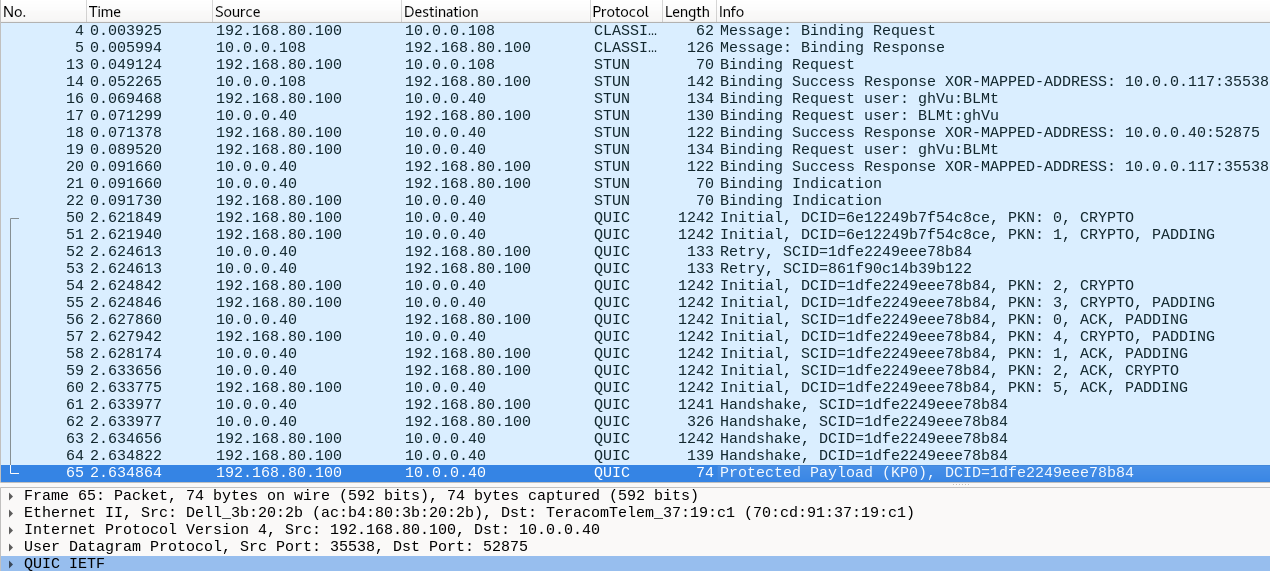
\includegraphics[width=0.90\linewidth]{fig/results/physical/gateway_a_pcap.png}
    \\ (a) \textit{Gateway} A
    
    \par\medskip

    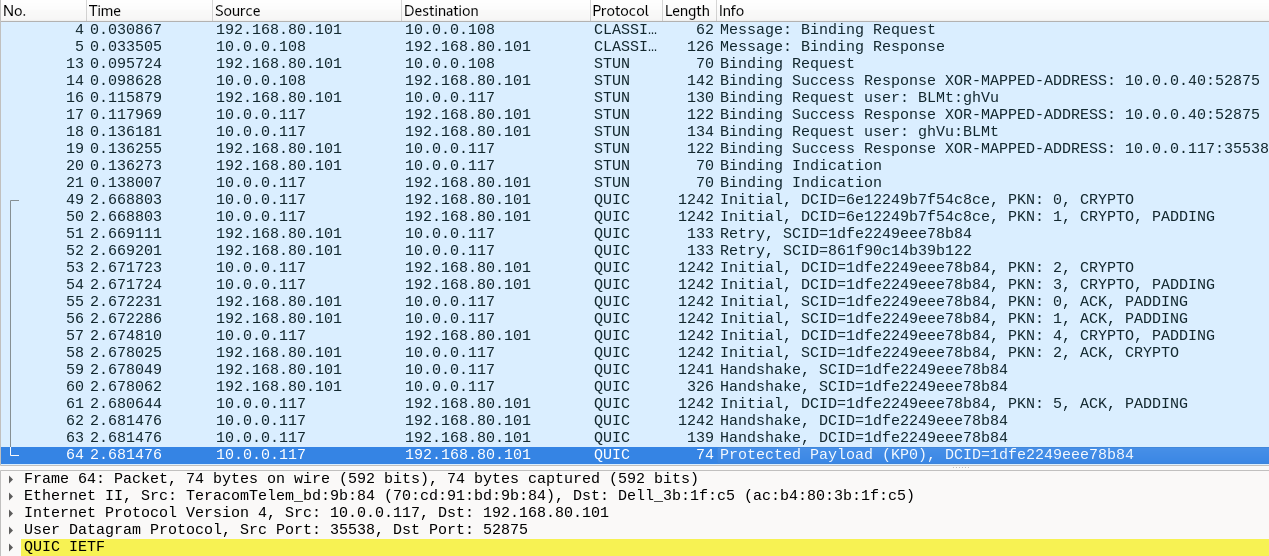
\includegraphics[width=0.90\linewidth]{fig/results/physical/gateway_b_pcap.png}
    \\ (b) \textit{Gateway} B

    \caption{Pacotes trocados no processo de conexão utilizando a infraestrutura física.}
    \label{fig:physical_connection_steps}
\end{figure}

Após o estabelecimento do QUIC, os dois \textit{gateways} registraram 16384 \textit{bytes} enviados e recebidos e a conclusão do encerramento. O gerador local também informou que a resposta do \textit{echo} era idêntica ao conteúdo enviado, seguida de EOF. A evidência de integridade vem dessa comparação byte a byte, e as capturas identificam o percurso e a sequência de protocolos utilizados.

\subsection{Comparação com o Ambiente PatchBay e Alcance dos Resultados}

Os resultados físicos mostram que o funcionamento observado no caso direto C10 do PatchBay (Seção~\ref{sec:functional_establishment}) também foi obtido com tradução e encaminhamento realizados por equipamentos externos. A mesma implementação integrou a negociação ICE, o transporte QUIC e as aplicações TCP locais nesse arranjo.

O alcance dessa observação se restringe à topologia e aos equipamentos utilizados. A coleta física analisada não exercita TURN obrigatório, sessão prolongada, perdas induzidas nem mudança de rede. Ela também não caracteriza sistematicamente o comportamento dos NATs nem estabelece diferenças de latência ou vazão em relação ao PatchBay. Esses aspectos exigiriam procedimentos e medições específicos, que ultrapassam o escopo deste trabalho.

\section{Análise Comparativa das Abordagens de Comunicação}
\label{sec:another_connection_approaches}

A análise conceitual contrapõe três abordagens para o mesmo tipo de comunicação:

\begin{itemize}
    \item a abordagem P2P com ICE e QUIC desenvolvida neste trabalho;
    \item a abordagem cliente-servidor, comum em aplicações IoT, na qual um servidor especializado intermedeia as conexões;
    \item uma abordagem P2P alternativa, com comunicação TCP estabelecida por TCP \textit{hole punching} (Seção~\ref{sec:tcp_hole_punching}).
\end{itemize}

\subsection{Comunicação P2P com ICE e QUIC}

A Figura~\ref{fig:non_centralized_quic_flow} apresenta o processo de conexão da abordagem P2P: a negociação ICE, o estabelecimento da conexão QUIC e, em seguida, as trocas diretas entre cliente e servidor.

\begin{figure}[!ht]
    \centering
    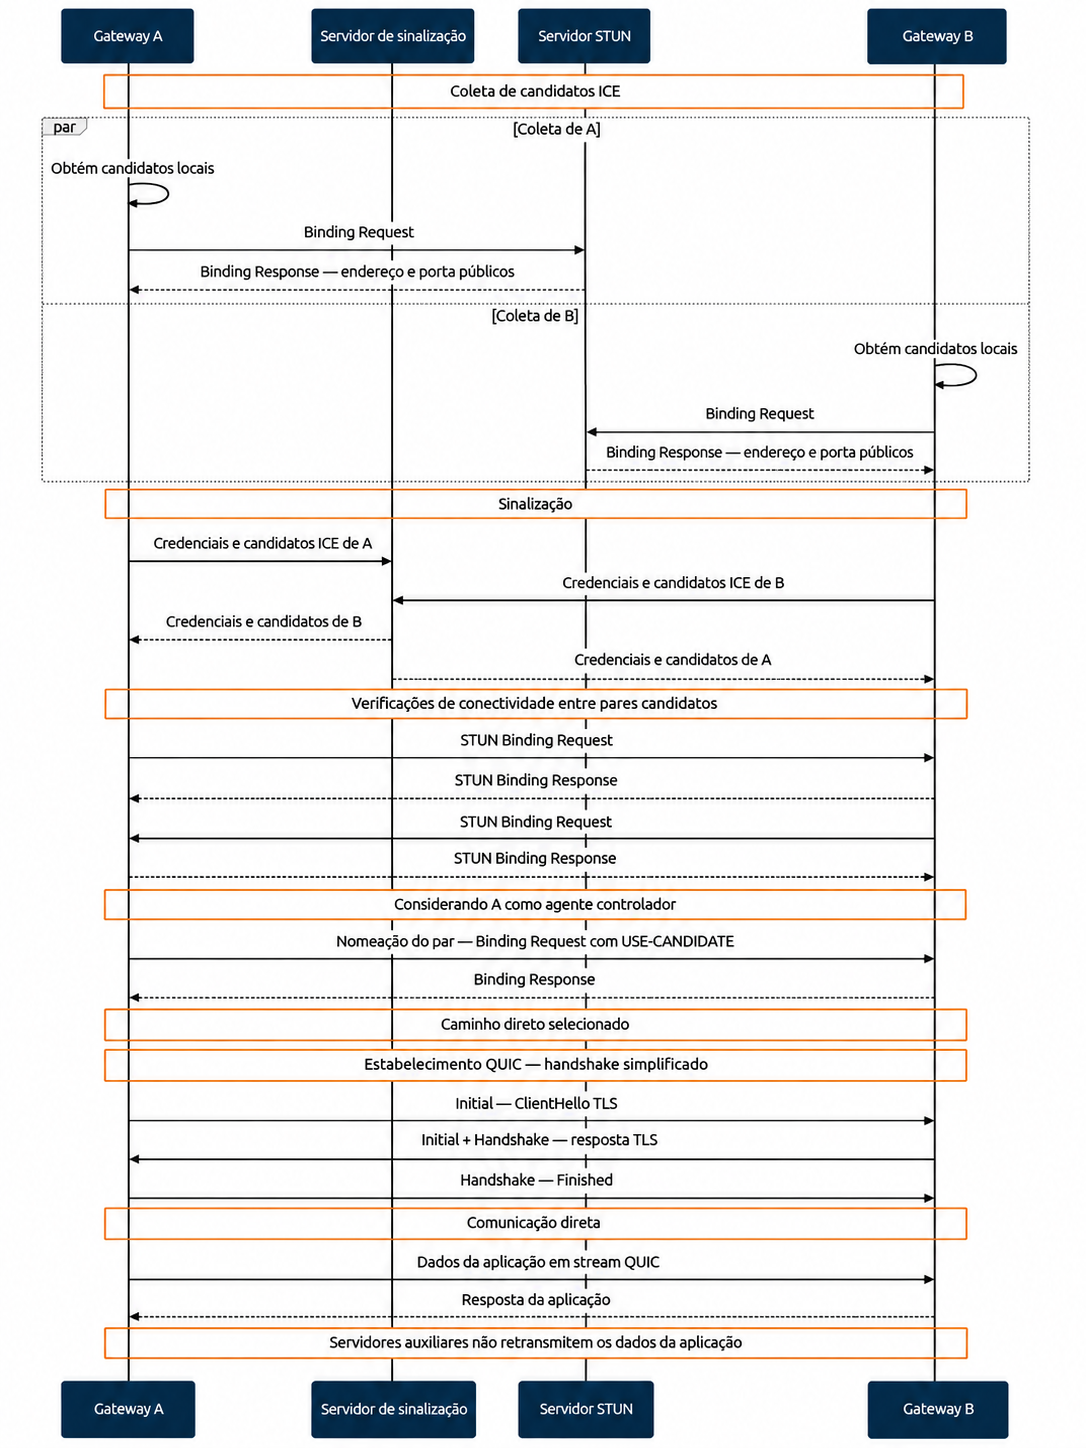
\includegraphics[width=0.7\textwidth]{fig/results/logic/flow_ice.png}
    \caption{Diagrama de tempo das etapas de comunicação com o ICE e o QUIC.}
    \label{fig:non_centralized_quic_flow}
\end{figure}

Quando o \textit{hole punching} falha e a comunicação recorre a um servidor TURN, o servidor passa a participar do estabelecimento, da manutenção da conexão e da troca de mensagens. Essa indireção acrescenta um custo à comunicação, semelhante ao da abordagem com servidor intermediário.

\subsection{Comunicação com Servidor Intermediário Especializado}

Nesta abordagem, o servidor especializado intermedeia toda a comunicação entre os \textit{peers}. A análise se concentra nas etapas de conexão e no custo lógico do envio de mensagens, mas a manutenção do servidor também representa um custo de infraestrutura. Os dois \textit{peers} se conectam ao servidor, que encaminha os pacotes entre eles. Supõe-se um cenário favorável, no qual a comunicação entre cada \textit{peer} e o servidor utiliza um protocolo que integra a confidencialidade ao estabelecimento da conexão, como o QUIC. Com TCP e TLS, o estabelecimento exigiria o \textit{3-way handshake} do TCP seguido do \textit{handshake} do TLS.

A Figura~\ref{fig:centralized_server_quic_flow} descreve as etapas dessa comunicação. Em comparação com o fluxo da Figura~\ref{fig:non_centralized_quic_flow}, a abordagem centralizada dispensa as etapas do ICE no estabelecimento da conexão. Em contrapartida, após o estabelecimento da conexão P2P, as mensagens trafegam diretamente entre os pares, enquanto a abordagem com servidor especializado mantém a indireção da retransmissão pelo servidor em todas as mensagens.

\begin{figure}[!ht]
    \centering
    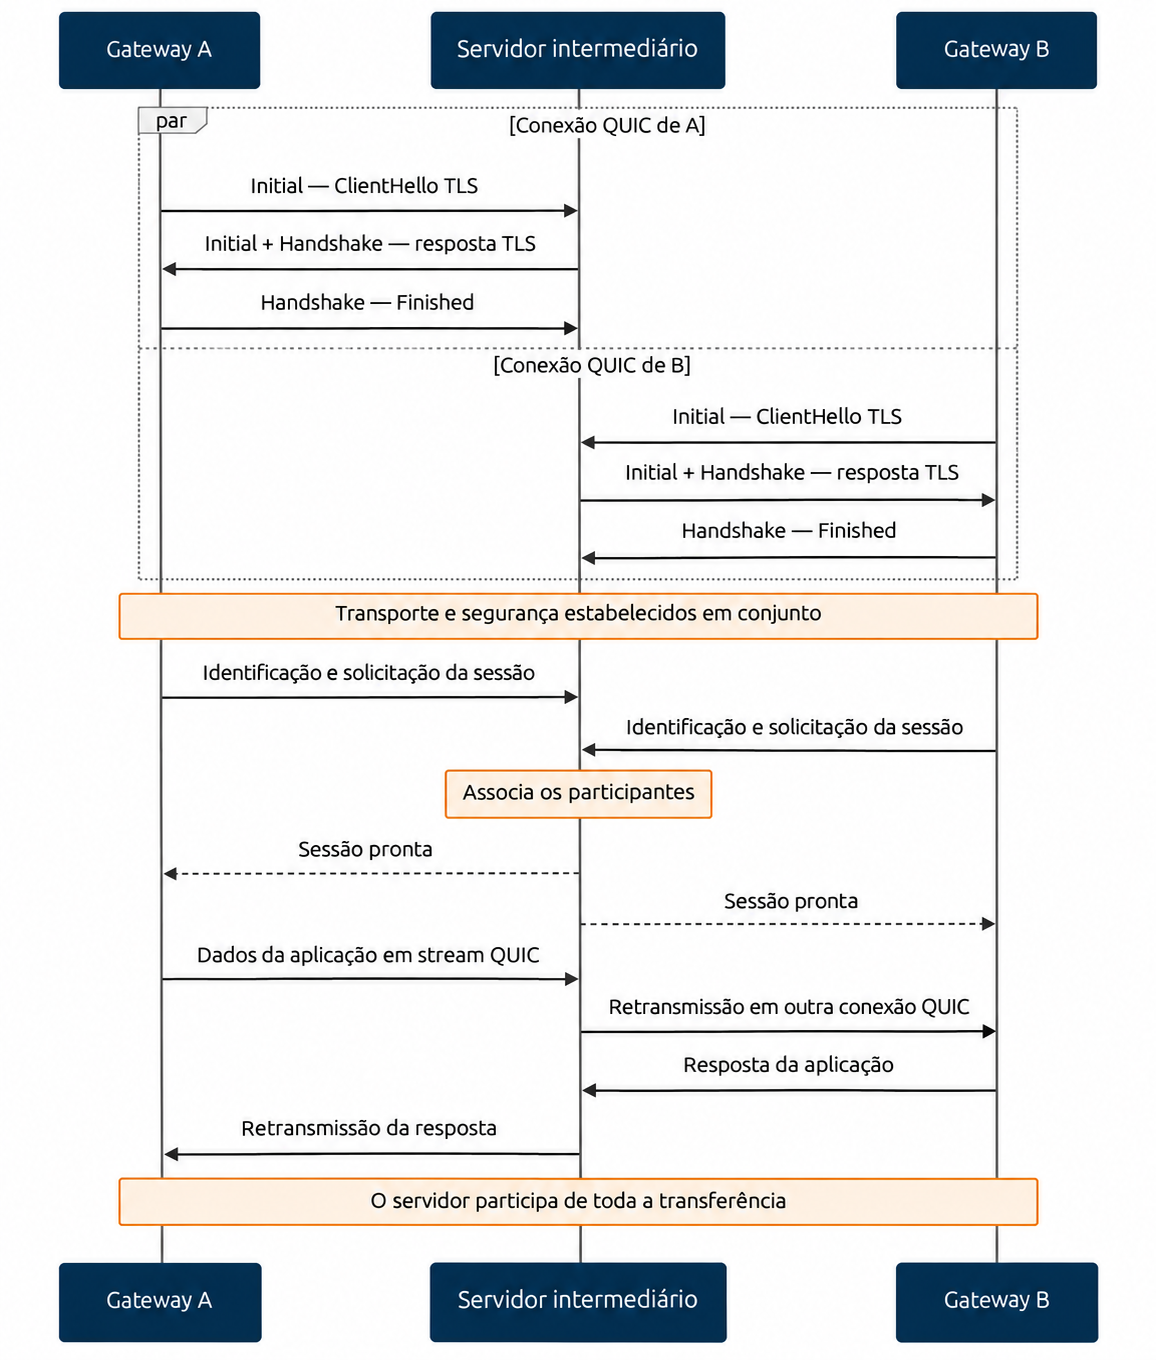
\includegraphics[width=0.7\textwidth]{fig/results/logic/centralized_server_quic_flow.png}
    \caption{Diagrama de tempo das etapas de comunicação utilizando um servidor especializado.}
    \label{fig:centralized_server_quic_flow}
\end{figure}

\subsection{Comunicação P2P com TCP Hole Punching}

Com o ICE sobre TCP, especificado no RFC~6544 \citep{rfc6544}, a comunicação entre os \textit{peers} segue um processo semelhante ao do ICE sobre UDP (Seção~\ref{sec:ice}). Entretanto, como o TCP não permite o envio de dados antes do estabelecimento da conexão, cada verificação de conectividade começa pela abertura de uma conexão TCP entre os candidatos, que pode ocorrer por abertura simultânea. Somente depois a transação STUN sobre essa conexão autentica o par e permite sua nomeação. A Figura~\ref{fig:non_centralized_ice_tcp_flow} apresenta esse fluxo.

\begin{figure}[!ht]
    \centering
    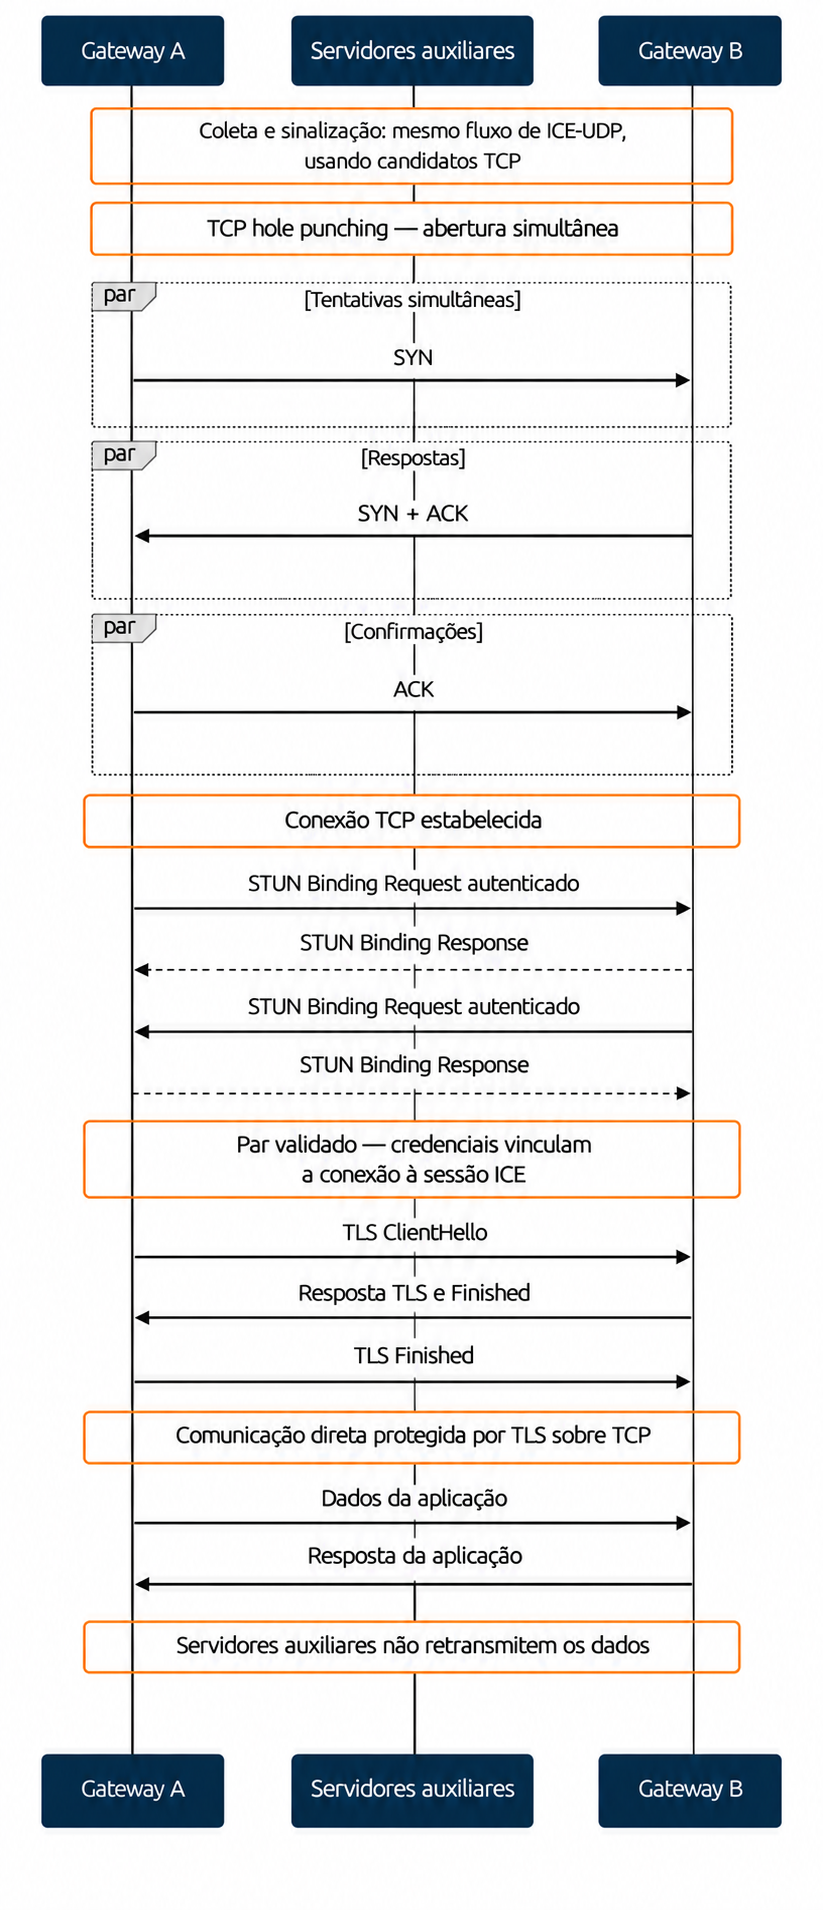
\includegraphics[width=0.5\textwidth]{fig/results/logic/flow_ice_tcp.png}
    \caption{Diagrama de tempo das etapas de comunicação utilizando ICE com TCP \textit{hole punching}.}
    \label{fig:non_centralized_ice_tcp_flow}
\end{figure}

\subsection{Comparação Conceitual entre as Abordagens}

Na conexão direta com o servidor (Figura~\ref{fig:centralized_server_quic_flow}), o próprio servidor tem acesso aos dados da aplicação, pois termina as sessões de transporte com os dois \textit{peers}. A cifragem protege os dados em trânsito em cada sessão, mas não oferece confidencialidade de ponta a ponta entre os \textit{peers} em relação ao servidor intermediário. Essa abordagem exige, portanto, uma camada adicional de proteção dos dados de aplicação, que a camada de transporte não provê. Esse problema não ocorre quando a abordagem P2P recorre a um servidor TURN. Nesse caso, a conexão QUIC permanece estabelecida de ponta a ponta entre os \textit{peers}, e o servidor TURN apenas retransmite os pacotes já cifrados.

Na abordagem centralizada, o servidor intermediário participa de toda a troca de dados, de modo que sua indisponibilidade interrompe a comunicação que depende dele. Na abordagem P2P, após o estabelecimento de um caminho direto, os dados trafegam entre os pares sem depender do servidor intermediário. Quando o caminho utiliza TURN, entretanto, o servidor \textit{relay} permanece necessário durante a sessão.

\citet{ford2005peer} observaram que a maioria dos dispositivos NAT avaliados admitia \textit{hole punching}, com taxas de sucesso de cerca de 82\% para UDP e 64\% para TCP. Esse resultado reduz a frequência com que as abordagens P2P precisam recorrer a um servidor \textit{relay}. Assim, a indireção, desvantagem da abordagem centralizada, ocorre na abordagem P2P apenas nos casos em que o \textit{hole punching} falha. Como essas medições datam de 2005, a proporção atual pode ser diferente, em particular em redes com NAT de operadora (CGNAT).

Com TCP \textit{hole punching}, o estabelecimento da comunicação inclui a abertura da conexão TCP antes da transação STUN de cada verificação de conectividade, conforme a Figura~\ref{fig:non_centralized_ice_tcp_flow}. Na abertura simultânea, os dois \textit{peers} estabelecem a mesma conexão TCP, e não duas conexões sequenciais. Para proteger os dados, a comunicação executa também o \textit{handshake} do TLS sobre a conexão estabelecida. Essas etapas distinguem essa abordagem da baseada em ICE sobre UDP seguido de QUIC, mas não determinam, por si só, o tempo total de estabelecimento em uma execução real.

Do ponto de vista operacional, o TCP expõe em texto claro os metadados da conexão, como os números de sequência e as \textit{flags}, o que permite a observação e a interferência de dispositivos intermediários. O QUIC, por outro lado, cifra seus quadros de controle e protege o número do pacote por meio da proteção de cabeçalho (Seção~\ref{sec:quic_header_protection}). Além disso, o TCP \textit{hole punching} exige cuidados adicionais com a abertura simultânea das conexões, a sincronização entre os pares e o comportamento dos \textit{sockets}, conforme discutido na Seção~\ref{sec:tcp_hole_punching}.